\documentclass[a4paper,11pt]{jsarticle}


% 数式
\usepackage{amsmath,amsfonts,amssymb}
\usepackage{bm}
\usepackage{physics}
% 画像
\usepackage[dvipdfmx]{graphicx}
% ローマ数字
\usepackage{otf}
% 単位
\usepackage{siunitx}
% 表
\usepackage{multirow}
% 化学反応
\usepackage[version=4]{mhchem}


\begin{document}

\title{理論演習4Sレポート}
\author{05-211525 齋藤駿一}
\date{\today}
\maketitle

\tableofcontents

\section{はじめに}
細胞内の代謝反応は様々な形でモデル化され,理論的に研究されてきた.
たとえば,非常に多数の成分からなる自己触媒反応ネットワークを考えることで,細胞内の分子数がZipfの法則に従うことが明らかになった\cite{hurusawa}.
ほかにも,代謝がある確率で失敗することでゴミ分子が生成され,それが正常な代謝を阻害するようなモデルも考えられた\cite{hk17}.
このモデルは,低栄養環境に置かれた細胞が高栄養環境に移されたときに成長を再開するのにかかる時間(ラグタイム)をよく説明することが分かった.
こうしたモデルは分子の詳細によらないため,様々な生体分子に関して普遍的に成り立つ法則を含んでいるといえる.

こうした研究を受け,私は,細胞が成長できる条件を分子の詳細によらない形で記述することを考えた.
具体的には,ごく簡単な自己触媒反応のモデルにより,栄養濃度がある閾値を下回ると細胞が成長できないことを明確に説明し,その閾値を解析的に導出した.
次に,このモデルの化学反応を若干変更した2つのモデルについて栄養濃度の閾値を再び求め,もとのモデルと比較して考察した.

なお,本レポートの内容の多くは解析的な議論であり,それは理論演習の授業がすべて終了した後に個人的に行ったものである.
そのため,授業で発表した数値計算の結果に対する考察は少なくなってしまった.
しかし,ここで扱っている細胞モデルは,基本的に授業で発表したモデルのいずれかと等価なので,授業と無関係ではないことをくみ取っていただければ幸いである.


\section{基本的な細胞モデル}
\subsection{セットアップ}
最初に,本レポートの中核をなす細胞モデルを構成する.
このモデルは,Himeoka and Kaneko (2014)のモデル\cite{hk14}をさらに簡単にしたものである.
まず,外部から栄養を取り込み成長する一つの細胞を考える.
この細胞は,外部の栄養分子N(濃度$n$)を取り込み,次の自己触媒反応により細胞内で代謝物X(濃度$x$)を生成する:
\begin{equation}
  \ce{N + X ->[$k$] X + X}.
\end{equation}
ただし,$k$はこの反応の速度定数である.
また,簡単のため,細胞膜における栄養分子の出入りは十分に素早く,細胞内の栄養濃度は細胞外の栄養濃度$n$に等しいと考える.
そのため,ここでは細胞内の栄養分子と細胞外の栄養分子を区別しないことにする.
次に,代謝物は反応速度$\phi$で消費されるとする:
\begin{equation}
  \ce{X ->[$\phi$] $\emptyset$}.
\end{equation}
そして,細胞の成長速度$\mu=V^{-1}dV/dt$($V$は細胞の体積)は代謝物Xの消費速度に比例すると考え,$\mu=\gamma \phi x$とする.
この$\mu$は成分の希釈率も意味する.

このとき,代謝物Xの濃度$x$は,微分方程式
\begin{equation}
  \frac{dx}{dt} = k n x - \phi x - \mu x
\end{equation}
に従う.
これはロジスティック方程式
\begin{equation}
  \frac{dx}{dt} = \gamma \phi x \left[\frac{1}{\gamma}\left(\frac{k}{\phi} n - 1\right) - x \right] \label{logistic}
\end{equation}
に書き換えられる.

ここでは,代謝物Xとして,細胞を構成する分子(たとえば細胞膜を作るリン脂質や細胞骨格など)を想定している.
そして,ここで言う「消費」とは,細胞質を拡散している分子が細胞の膜や骨格として固定されることを指している.
しかしその一方で,代謝物Xを,ある速度で分解するリボソームと捉えても良い.
その場合,分解速度は$\phi$であり,成長速度$\mu$はリボソーム濃度$x$に比例する(比例係数$\gamma\phi$),と解釈することができる.
また,このような現実の細胞との対応という観点で言えば,代謝物Xを生成する自己触媒反応は,実際の代謝反応をかなり簡単に捉えたものにすぎない.

\subsection{結果と考察}
方程式\eqref{logistic}の定常解のうち安定なものは,栄養濃度$n$によって
\begin{equation}
  \begin{cases}
    \frac{k}{\phi} n - 1 > 0 \text{のとき} & x = \frac{1}{\gamma} \left( \frac{k}{\phi} n - 1 \right) \\
    \frac{k}{\phi} n - 1 < 0 \text{のとき} & x = 0
  \end{cases}
\end{equation}
と分岐(トランスクリティカル分岐)する.
したがって,成長速度が正,つまり$x > 0$であるには,栄養濃度$n$は$n > n^* = \phi/k$を満たす必要がある.
つまり,細胞が成長できる栄養濃度には下限が存在し,それは代謝物の消費反応の速度定数を生成反応の速度定数で割った値に等しい.

また,一般に成長速度$\mu$が代謝物濃度$x$の単調増加関数$\mu(x)$である場合にも,$\mu(0)=0$(代謝物が存在しないとき細胞は成長しないという条件)が成り立つならば,まったく同じことがいえる.
実際,この場合には方程式\eqref{logistic}のかわりに
\begin{equation}
  \frac{dx}{dt} =  x \left(kn - \phi - \mu(x)\right) 
\end{equation}
が成り立ち,安定な定常解は
\begin{equation}
  \begin{cases}
    \frac{k}{\phi} n - 1 > 0 \text{のとき} & x = \mu^{-1}\left(kn - \phi \right) >0 \\
    \frac{k}{\phi} n - 1 < 0 \text{のとき} & x = 0
  \end{cases}
\end{equation}
となる.ただし,$\mu(x)$の逆関数を$\mu^{-1}(x)$とした.


\section{細胞内外で栄養濃度が異なるモデル}
\subsection{セットアップ}
先ほどのモデルでは,細胞内の栄養濃度は細胞外の栄養濃度と等しい定数であると考えていた.
しかし実際には,細胞内の栄養濃度は,細胞外からの栄養分子の流入と細胞内での反応による消費によって変動する量と考えるべきである.
そこで次に,細胞外の栄養濃度のみを定数とし,細胞内の栄養濃度を変数としたモデルを考える.
つまり,細胞外の栄養分子をN,細胞内の栄養分子をYとしたとき,拡散(拡散係数$D$)による流出入
\begin{equation}
  \ce{N <->[$D$] Y}
\end{equation}
を考え,自己触媒反応として
\begin{equation}
  \ce{Y + X ->[$k$] X + X}
\end{equation}
を考える.
代謝物Xの消費とそれによる細胞の成長は,先ほどと同様に考える.

このとき,細胞内の栄養濃度を$y$として,方程式\eqref{logistic}は
\begin{equation}
  \frac{dx}{dt} = \gamma \phi x \left[\frac{1}{\gamma}\left(\frac{k}{\phi} y - 1\right) - x \right] 
\end{equation}
と書き換えられる.
一方,細胞内の栄養濃度$y$に関する微分方程式は,細胞外の栄養濃度$n$を用いて
\begin{equation}
  \frac{dy}{dt} = D(n-y) - kxy - \mu y.
\end{equation}
と書ける.
これは
\begin{equation}
  \frac{dy}{dt} = Dn - \left[ D + \left(k + \gamma \phi \right)x \right]y
\end{equation}
と書き換えられる.
さらに,これらの$x,y$に関する微分方程式は,
\begin{equation}
  \tilde{x} = \frac{k + \gamma \phi}{D}x,\qquad \tilde{y} = \frac{k}{\phi} y, \qquad \tilde{t} = Dt
\end{equation}
と変数変換することで,次のように無次元化することができる:
\begin{align}
  \frac{d\tilde{x}}{d\tilde{t}} &= \alpha \tilde{x} \left[ \beta \left( \tilde{y} - 1 \right) - \tilde{x} \right] \label{ndx}\\
  \frac{d\tilde{y}}{d\tilde{t}} &= \frac{kn}{\phi} - \left( \tilde{x} + 1\right)\tilde{y}. \label{ndy} 
\end{align}
ただし,
\begin{equation}
  \alpha = \frac{\gamma\phi}{k + \gamma\phi},\qquad \beta = \frac{k + \gamma\phi}{\gamma D}
\end{equation}
とおいた.

\subsection{結果と考察}
この細胞モデルでも,先ほどとまったく同様に,成長条件が$n>\phi/k$となることが示せる.
その証明は以下の通りである.

無次元化した方程式\eqref{ndx},\eqref{ndy}の定常解で$\tilde{x}, \tilde{y} \ge 0$を満たすものは,
\begin{equation}
  \begin{cases}
    \frac{k}{\phi} n > 1 \text{のとき} & (\tilde{x},\tilde{y}) = \left(0, \frac{kn}{\phi}\right),\, \left(\tilde{x}^*, \tilde{y}^*\right) \\
    \frac{k}{\phi} n < 1 \text{のとき} & (\tilde{x},\tilde{y}) = \left(0, \frac{kn}{\phi}\right)
  \end{cases}
\end{equation}
である.ただし,
\begin{equation}
  \tilde{x}^* = \frac{\sqrt{(\beta-1)^2+4\beta kn/\phi} - (\beta+1)}{2}, \qquad \tilde{y}^* = \frac{\sqrt{(\beta-1)^2+4\beta kn/\phi} + (\beta-1)}{2\beta}
\end{equation}
とおいた.
これらの定常解の安定性を調べるため,$(\tilde{x}, \tilde{y})$におけるヤコビ行列を計算すると,
\begin{equation}
  J = \begin{pmatrix}
    \alpha\beta (\tilde{y} -1) -2\alpha \tilde{x} & \alpha\beta \tilde{x} \\
    - \tilde{y} & - \tilde{x} - 1 \\
    \end{pmatrix}
\end{equation}
となる.
まず,$(\tilde{x}, \tilde{y}) = (\tilde{x}^*, \tilde{y}^*)$において,ヤコビ行列の固有値を計算すると,
\begin{equation}
  \lambda = \frac{-(\alpha \tilde{x}^* + \tilde{x}^* + 1) \pm \sqrt{(\alpha \tilde{x}^* + \tilde{x}^* + 1)^2 - 4\alpha \tilde{x}^* (\tilde{x}^* + \beta\tilde{y}^* + 1)}}{2}
\end{equation}
と求まる.
根号の中身が非負のとき,固有値は二つの負の実数となり,根号の中身が負のとき,固有値は実部が負となる二つの複素数となる.
よって,常に固有値$\lambda$の実部は負となるので,定常解$(\tilde{x}, \tilde{y}) = (\tilde{x}^*, \tilde{y}^*)$は安定である.
一方で,$(\tilde{x}, \tilde{y}) = (0, kn/\phi)$においては,固有値は
\begin{equation}
  \lambda = -1,\,\alpha \beta \left(\frac{kn}{\phi} - 1\right)
\end{equation}
と求まる.
よってこの定常解は,$kn/\phi < 1$のとき安定,$kn/\phi > 1$のとき不安定となる.
以上より,安定な定常解は次のようになる:
\begin{equation}
  \begin{cases}
    \frac{k}{\phi} n > 1 \text{のとき} & (\tilde{x},\tilde{y}) = \left(\tilde{x}^*, \tilde{y}^*\right) \\
    \frac{k}{\phi} n < 1 \text{のとき} & (\tilde{x},\tilde{y}) = \left(0, \frac{kn}{\phi}\right).
  \end{cases}
\end{equation}
したがって,成長速度が正,つまり$\tilde{x} > 0$であるには,やはり$n > n^* = \phi/k$が必要となる.
これは,細胞内外で栄養濃度が共通であると考えた先ほどのモデルと同じ結果である.


\section{ゴミ分子を導入したモデル}
\subsection{セットアップ}
次に,Himeoka and Kaneko (2017)のモデル\cite{hk17}を参考に,代謝物Xを生成する反応が失敗しうるモデルを考えた.
まず,代謝物Xを作る反応において,ある確率$\epsilon$でエラーが発生し,ゴミ分子Zができると仮定する.
さらに,ゴミ分子Zは代謝物Xと可逆的に結合し,複合体Cを作ると仮定する.
これは,代謝物Xの自己触媒を阻害する反応である.
つまり,以下の拡散および反応を考える:
\begin{align}
  \ce{N &<->[$D$] Y} \\
  \ce{Y + X &->[$k(1-\epsilon)$] X + X} \\
  \ce{Y + X &->[$k\epsilon$] Z + X} \\
  \ce{Z + X &<=>[$k_1$][$k_2$] C} \\
  \ce{X &->[\phi] \emptyset}.
\end{align}
よって,化学種X,Y,Z,Cの濃度をそれぞれ$x,y,z,c$とおくと,方程式は次のようになる:
\begin{align}
  \frac{dx}{dt} &= k(1-\epsilon)xy - k_1 xz + k_2 c - \phi x - \mu x\\
  \frac{dy}{dt} &= D(n-y) - kxy - \mu y \\
  \frac{dz}{dt} &= k\epsilon xy - k_1 xz + k_2 c - \mu z \\
  \frac{dc}{dt} &= k_1 xz - k_2 c - \mu c \\ 
  \mu &= \gamma \phi x.
\end{align}

\subsection{結果と考察}
\subsubsection{エラー率が一定の場合}
まず,$\epsilon$が定数である場合を考える.
このとき,成長条件は$n > n^* = \phi/(k(1-\epsilon))$であることが次のように示せる.

まず,微分方程式で$d/dt=0$として得られる代数方程式から
\begin{align}
  y &= \frac{n}{1+\frac{k+\gamma\phi}{D}x} \\
  c &= \frac{k_1xz}{k_2+\gamma\phi x}
\end{align}
が導かれる.
これを用いて,同様に得られる残り2本の代数方程式から$c$を消去すると,$x\neq 0$なる定常解に対して
\begin{align}
  z &= \frac{\phi(1+\gamma x) - k(1-\epsilon)y}{\frac{k_1k_2}{k_2+\gamma\phi x} - k_1} \\
  z &= \frac{-k\epsilon y}{\frac{k_1k_2}{k_2+\gamma\phi x} - k_1 - \gamma\phi}
\end{align}
がそれぞれ導かれる.
さらに,この二つが等しいとした式から$y$を消去することで,Xの濃度$x$の0以外の定常解は
\begin{equation}
  1-\epsilon \left[1 + \left(\frac{k_2}{k_1 x} + 1 - \frac{\gamma \phi}{k_1}\right)^{-1} \right] = \frac{\phi}{kn}(1+\gamma x)\left(1+\frac{k+\gamma\phi}{D}x\right)
\end{equation}
を満たすと分かる.
さらに$x \ge 0$において,左辺は$x$とともに減少し,右辺は$x$とともに増加することから,定常解$x>0$が存在する条件は,
\begin{equation}
  1-\epsilon > \frac{\phi}{kn}
\end{equation}
と分かる.
したがって,栄養濃度の満たすべき条件は
\begin{equation}
  n > n^* = \frac{\phi}{k(1-\epsilon)} \label{nast_errconst}
\end{equation}
と求まる.

この式は,代謝物Xの消費反応の速度定数が$\phi$,生成反応の実効的な速度定数が$k(1-\epsilon)$となることから説明できる.
また,反応$\ce{Z + X <=> C}$はここでは効いていないことが分かる.

しかし,この証明のような解析的な手法では,式\eqref{nast_errconst}が成り立つときに$x>0$を満たす定常解が安定であること(成長速度が正の値で安定すること)を示すのが難しかった.
そこで次に,数値計算によって式\eqref{nast_errconst}と成長速度が正であることが等価であることを部分的に確認した.
ここでは,パラメータ$k,k_1,k_2,\phi,\gamma,D$はすべて1とした.
まず,外部栄養濃度$n$をある値に固定し,$\epsilon=0,0.2,0.4,0.6,0.8$のそれぞれについて,初期濃度を$x=y=1, z=c=0$として十分な時間(時刻$t=10^5$まで)シミュレーションを行った.
その結果,最終的にすべての成分濃度と成長速度$\mu$が定常となっていることを確認した.
このとき,外部栄養濃度$n$と定常成長速度$\mu$の関係は図\ref{fig:n_vs_mu_errconst}のようになった.
この図を参考に,定常成長速度が$\mu > 10^{-3}$となる最小の外部栄養濃度$n^*$を「成長に必要な栄養濃度」と考えることにした.
そこで,外部栄養濃度$n$を0から0.1ずつ増加させ,$\mu>10^{-3}$となる最小の$n$を$n^*$として,$\epsilon$と$n^*$の関係をプロットした(図\ref{fig:err_vs_n_errconst}).
この図から,理論式\eqref{nast_errconst}はこの数値計算の結果と整合することが確認できる.

\begin{figure}[htbp]
  \centering
  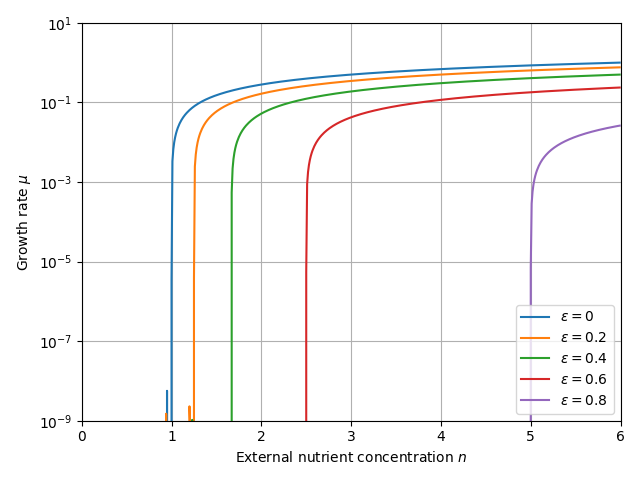
\includegraphics[width=10cm]{n_vs_mu_errconst.png}
  \caption{エラー率を定数($\epsilon=0,0.2,0.4,0.6,0.8$)として計算した,時刻$t=10^5$における外部栄養濃度$n$と成長速度$\mu$の関係(初期濃度は$x=y=1, z=c=0$,時間の刻み幅は0.1,$n$の刻み幅は0.01,その他のパラメータ$k,k_1,k_2,\phi,\gamma,D$はすべて1とした.).この結果は式\eqref{nast_errconst}と整合する.}
  \label{fig:n_vs_mu_errconst}
\end{figure}

\begin{figure}[htbp]
  \centering
  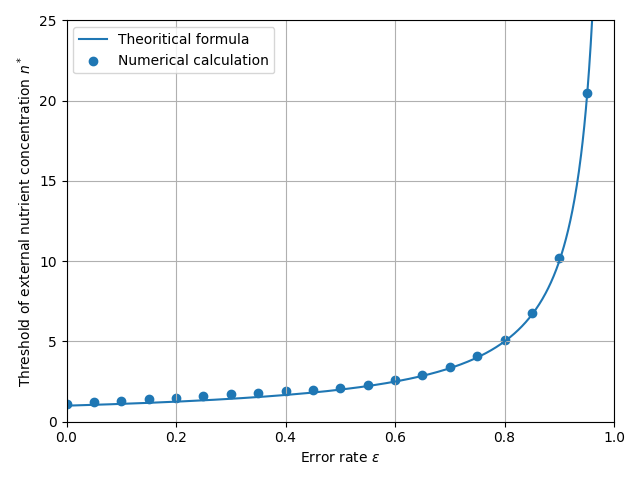
\includegraphics[width=10cm]{err_vs_n_errconst.png}
  \caption{エラー率が定数であるとして計算した,$\epsilon$と成長に必要な($\mu > 10^{-3}$となる最小の)外部栄養濃度$n^*$の関係(Numerical calculationとして示したプロット.$n^*$を求めるにあたって,$n$は刻み幅0.1で変更した.それ以外のパラメータは図\ref{fig:n_vs_mu_errconst}と同様である.).これは式\eqref{nast_errconst}で表される理論線(Theoritical formulaとして示した曲線)と整合している.}
  \label{fig:err_vs_n_errconst}
\end{figure}

\subsubsection{エラー率が代謝物濃度$x$に依存する場合}
次に,エラー率$\epsilon$が変化する場合を考える.
まず,ここでは代謝物濃度$x$に依存して
\begin{equation}
  \epsilon = \frac{\delta}{K + x} \label{errx}
\end{equation}
と書ける場合を考える.
ただし,エラー率は0以上1以下の値をとるので,$0 \le \delta \le K$とする.
なお,この式の形は,Himeoka and Kaneko (2017)のモデル\cite{hk17}を参考に,代謝物Xが多いときにエラー率が低くなるようにした.

この場合には,解析的に定常解を求めることがやや困難なので,数値計算の結果をもとに考察を行う.

まず,$K=1$とし,$\delta=0,0.2,0.4,0.6,0.8,1$のそれぞれについて,先ほどと同様にシミュレーションを行った.
その結果,外部栄養濃度$n$と定常成長速度$\mu$の関係は図\ref{fig:n_vs_mu_K1s0}のようになった.
この図を参考に,定常成長速度が$\mu > 10^{-3}$となる最小の外部栄養濃度$n^*$を「成長に必要な栄養濃度」と考えた.
そして,$K=0.1,0.5,1$のそれぞれについて,$\delta/K$と$n^*$の関係をプロットした(図\ref{fig:err_vs_n_errslope_s0}).
また,同図に$\epsilon=\delta/K$で一定としたときの理論線(式\eqref{nast_errconst})も記載した.
これらを比較すると,$\delta/K$が小さいときのプロットは理論線と重なっているが,$\delta/K$が大きいときは理論線とずれて,$n^*$が発散しなくなることが分かった.
また,理論線から外れ始める$\delta/K$の値は,$K$とともに増加することも分かった.

次にその理由を考察する.
まず$\delta/K$が小さいとき,エラー率が低いため$n^*$は小さく済む.
これに伴い,$n\approx n^*$において$x \ll K$が成り立つ.
(いま,$\gamma=\phi=1$として計算しているので,$\mu=x$が成り立つ.つまりこの主張は,図\ref{fig:n_vs_mu_K1s0}の縦軸を,$n\approx n^*$におけるXの濃度$x$と読み替えることで確認できる.)
そのため,式\eqref{errx}より$\epsilon \approx \delta/K$と考えて良い.
よって,エラー率が$\delta/K$で一定と考えた場合と結果が一致すると考えられる.
逆に,$\delta/K$が大きいとき,$x$が$K$に対して無視できず,$x$が大きいほどエラー率が$\delta/K$よりも小さくなることで,$n^*$が小さく済むと考えられる.
さらに,$K$が大きい方が$x \ll K$となりやすいので,$\epsilon=\delta/K$の曲線から外れづらくなると説明できる.

\begin{figure}[htbp]
  \centering
  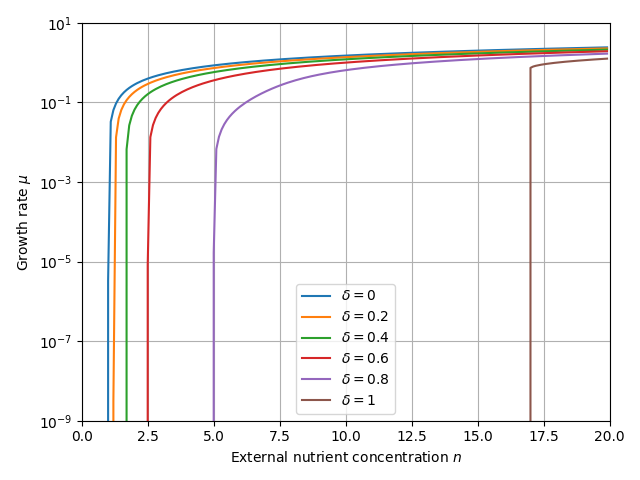
\includegraphics[width=10cm]{n_vs_mu_K1s0_errslope_all.png}
  \caption{エラー率が$x$に式\eqref{errx}の形($K=1$,$\delta=0,0.2,0.4,0.6,0.8,1$)で依存するとして計算した,時刻$t=10^5$における外部栄養濃度$n$と成長速度$\mu$の関係($n$の刻み幅を0.1に変更した.それ以外のパラメータは図\ref{fig:n_vs_mu_errconst}と同様である.).この結果を見ると,$\delta=1$以外は,$\epsilon=\delta/K$とみなしたときの図\ref{fig:n_vs_mu_errconst}と変わらないことが分かる.}
  \label{fig:n_vs_mu_K1s0}
\end{figure}

\begin{figure}[htbp]
  \centering
  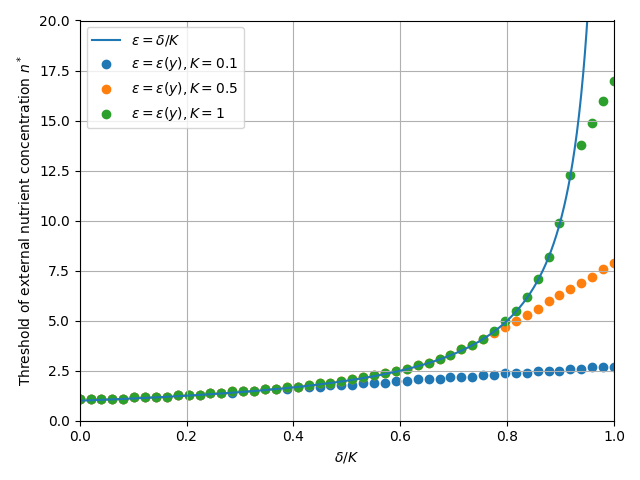
\includegraphics[width=10cm]{err_vs_n_errslope_s0_K.png}
  \caption{エラー率が$x$に式\eqref{errx}の形($K=0.1,0.5,1$)で依存するとして計算した,$\delta$と成長に必要な($\mu > 10^{-3}$となる最小の)外部栄養濃度$n^*$の関係($n$は刻み幅0.1で変更した.それ以外のパラメータは図\ref{fig:n_vs_mu_errconst}と同様である.).これを$\epsilon=\delta/K$のときの理論線と比較すると,$\delta/K$が大きくなるにつれて差が広がることが分かる.また,プロットが理論線から外れ始める$\delta/K$の値は,$K$とともに増加する.}
  \label{fig:err_vs_n_errslope_s0}
\end{figure}

\subsubsection{エラー率が内部栄養濃度$y$に依存する場合}
次に,エラー率が細胞内の栄養濃度$y$に依存して
\begin{equation}
  \epsilon = \frac{\delta}{K + y} \label{erry}
\end{equation}
と書ける場合を考える.
この場合に,$K=1$として同様の数値計算を行い,$\delta$と定常成長速度$\mu$の関係をプロットした(図\ref{fig:n_vs_mu_K1s1}).
次に,この図を参考に,成長に必要な外部栄養濃度$n^*$をこれまでとまったく同じように定義した.
そして,$K=1,10,100$のそれぞれについて,$\delta/K$と$n^*$の関係をプロットした(図\ref{fig:err_vs_n_errslope_s1}).
この図からも,図\ref{fig:err_vs_n_errslope_s0}と同じく,$\delta/K$が大きくなると理論線(式\eqref{nast_errconst}で$\epsilon=\delta/K$としたもの)から外れることと,$K$が大きいとプロットが理論線から外れ始める$\delta/K$の値が大きくなることが読み取れる.
それらについての考察は同様なので省略する.

一方で,図\ref{fig:err_vs_n_errslope_s0}と図\ref{fig:err_vs_n_errslope_s1}を比べると,同じ$K$の値に対し,エラー率が$x$に依存しているときに比べて,$y$に依存しているときの方が$n^*$が小さく済むことが読み取れる.
これについては,以下のように説明ができる.
まず,成長できる最小限近くの外部栄養濃度$n\approx n^*$において,$\mu$が小さいことから$x$は小さい.
その一方で,$y$は拡散流入により$n^*$近くの値になる.
つまり,$x$より$y$の方が大きいため,エラー率は式\eqref{errx}よりも式\eqref{erry}の方が小さくなる.
その結果,エラー率が$y$に依存する場合の方が$n^*$が少なく済むと考えられる.

\begin{figure}[htbp]
  \centering
  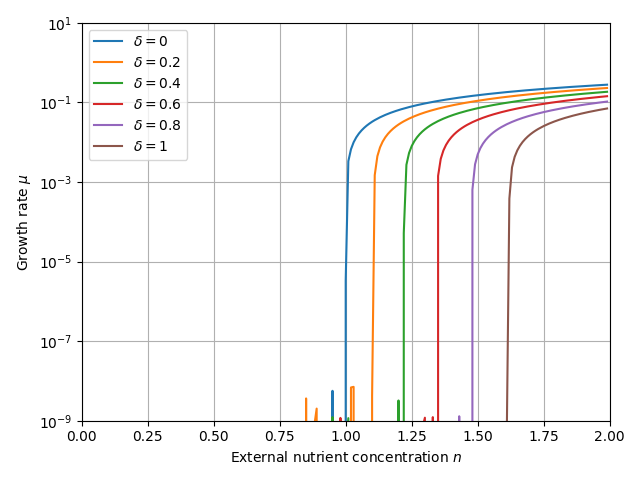
\includegraphics[width=10cm]{n_vs_mu_K1s1_errslope.png}
  \caption{エラー率が$y$に式\eqref{erry}の形($K=1$,$\delta=0,0.2,0.4,0.6,0.8,1$)で依存するとして計算した,時刻$t=10^5$における外部栄養濃度$n$と成長速度$\mu$の関係(刻み幅,初期濃度,パラメータの取り方は図\ref{fig:n_vs_mu_errconst}のときと同様である.).この場合,エラー率が$x$依存する場合と比べて,成長に必要な$n$は少なく済む.}
  \label{fig:n_vs_mu_K1s1}
\end{figure}

\begin{figure}[htbp]
  \centering
  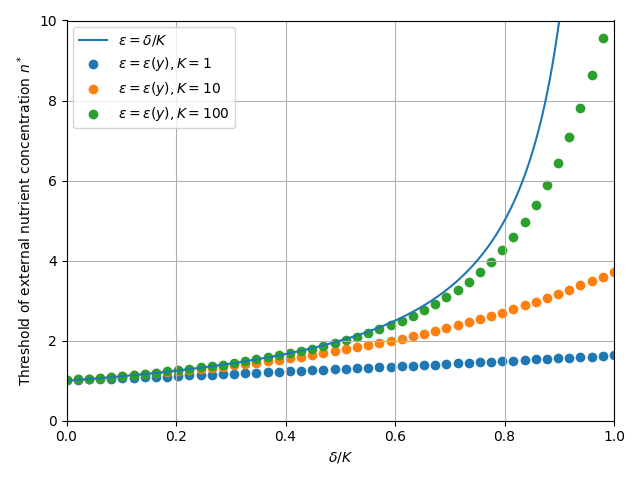
\includegraphics[width=10cm]{err_vs_n_errslope_s1_K.png}
  \caption{エラー率が$y$に式\eqref{erry}の形($K=1,10,100$)で依存するとして計算した,$\delta$と成長に必要な($\mu > 10^{-3}$となる最小の)外部栄養濃度$n^*$の関係($n$は刻み幅0.01で変更した.それ以外のパラメータは図\ref{fig:n_vs_mu_errconst}と同様である.).}
  \label{fig:err_vs_n_errslope_s1}
\end{figure}



\section{結論と今後の課題}
本レポートでは,ある栄養濃度以下で成長速度が急激に下がるという現象を,代謝物Xの生成,消費,希釈の三つの要因により説明した.
とくに,この三つの要因だけを反映した簡単な細胞モデルから,成長に必要な栄養濃度$n^*$は,代謝物Xの消費反応の速度定数$\phi$を生成反応の速度定数$k$で割った値$\phi/k$であることが分かった.
さらに,細胞内の栄養濃度を変数としたモデルでも,まったく同じ主張が成り立つことが分かった.
そのほかに,代謝物Xの生成反応が確率$\epsilon$で失敗してゴミ分子Zを生成し,それによって代謝物Xの自己触媒反応が阻害されるというモデルも考えた.
その場合,$\epsilon$が成分濃度によらず一定ならば,実効的な生成反応$k(1-\epsilon)$を$k$の代わりに使った値$\phi/(k(1-\epsilon))$が$n^*$となることが分かった.
さらに,エラー率が成分濃度に依存する場合でも,$n^*=\phi/(k(1-\epsilon))$をもとに,数値計算の結果をある程度説明できた.
つまり,最初のモデルで得られた式$n^*=\phi/k$は,細胞の成長条件を調べる一つの方法として有効だと考えられる.

しかし,自己触媒反応$\ce{N(Y) + X -> X + X}$に変更を加えた場合の議論や,エラー率が式\eqref{errx},\eqref{erry}以外の形で成分濃度に依存するときの議論などはまだ行っていない.
また,一般にどのような化学反応系で本レポートと同じような議論ができるかという問題も残っている.
とくに最後の問題にはっきりと答えるには,本レポートの議論をさらに数学的に洗練された形に言い換える必要があると思われる.
このような残された問題については,今後探求していきたい.

\begin{thebibliography}{99}
  \bibitem{hurusawa} Hurusawa, C. and Kaneko, K. Zipf's Law in Gene Expression. \textit{Phys. Rev. Lett.} \textbf{90}: 088102, 2003.
  \bibitem{hk17} Himeoka, Y. and Kaneko, K. Theory for Transitions Between Exponential and Stationary Phases:
  Universal Laws for Lag Time. \textit{Phys. Rev. X.} \textbf{7}: 021049, 2017.  
  \bibitem{hk14} Himeoka, Y. and Kaneko, K. Entropy production of a steady-growth cell with catalytic reactions. \textit{Phys. Rev. E.} \textbf{90}: 042714, 2014.  
\end{thebibliography}

\end{document}